\documentclass[11pt,twoside]{article}
%加载中文环境
\usepackage{ctex}

%插入图片
\usepackage{graphicx}

%字母加黑
\usepackage{bm}
% 插入公式的环境
\usepackage{amsmath}
\usepackage{amsfonts}
\usepackage{amssymb}

%是的图片的编号与章节关联
\counterwithin{figure}{section}
\usepackage[lmargin = 1in, rmargin = 1in, tmargin = 1in, bmargin = 1in]{geometry}

%cover information


% -------------------
% Content
% -------------------
\begin{document}
\section{基本方程}
\subsection{流体微团与随体导数}
这里的基本方程主要为对质量守恒,动量守恒,能量守恒方程的推导。

推导的是建立在流体质点或者流体微团的假设基础之上,我们认为流体为连续介质,其中最小的为流体质点和流体微团,流体质点为可以代表流体基本性质
的代表点,包括流体密度,流体单位质量的包含动量,流体单位质量包含能量三个。我们使用图1.1说明流体微团的意义。
\begin{figure}[htbp]
    \begin{center}
        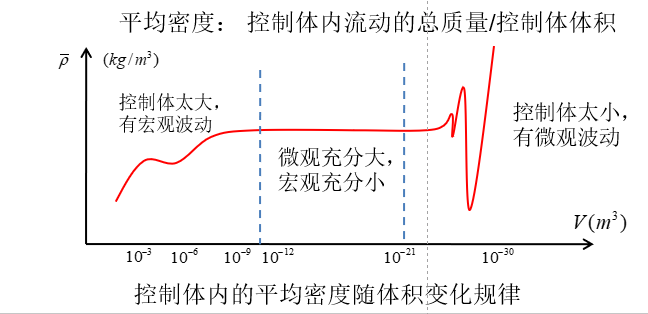
\includegraphics{流体质点.jpg}
    \end{center}
    \caption{控制体内平均密度随着体积变化规律}
\end{figure}

这里给出三种物理量的表示方法:

质量密度$\rho$:单位体积内的质量大小

动量密度$\bm{\theta}$ :单位体积内质量所携带的动量大小

能量密度$E$: 单位体积内物体所携带的能量大小

三者的表达式分别为:

质量密度为:$\rho$

动量密度为:$\bm{\theta} = \rho\times \bm{V}$

能量密度:$E = C_v \rho T + 1/2 \rho (w^2 + u^2 + v^2)$

这里需要解释的是,动量为矢量,我们在计算的过程中需要考虑方向,而能量与质量为标量。另外这里的$C_v$为单位质量的某物质温度升高$1k$所需要吸收的热量。
从而可以说明能量密度中前者所指的为内能,后者为动能,$w,u,v$分别是微团$x,y,z$三个方向的速度分量。

另外一个需要说明的为随体导数。对流体描述有欧拉法和拉格朗日法,每个流体质点的物理量是随着时间和位置发生变化的
流体微团的物理量可以用$f(x,y,z,t)$,则根据全微分的方法有:
$$df(x,y,z,t) = \frac{\partial f}{\partial x} dx + \frac{\partial f}{\partial y} dy + \frac{\partial f}{\partial z} dz + \frac{\partial f}{\partial t} dt$$

在公式的两边同时除以$dt$就可以得到:

$$\frac{df}{dt} = \frac{\partial f}{\partial x} \frac{dx}{dt} + \frac{\partial f}{\partial y} \frac{dy}{dt} + \frac{\partial f}{\partial z} \frac{dz}{dt} + \frac{\partial f}{\partial t}$$

其中的$\frac{dx}{dt},\frac{dy}{dt},\frac{dz}{dt}$分别为$x,y,z$方向的速度分量,可以用矢量$\bm{V}$表示。另外
令$\nabla = \frac{1}{\partial x} + \frac{1}{\partial y} +\frac{1}{\partial z}$为拉普拉斯算子。所以就可以得到随体导数的公式:

$$\frac{df}{dt} = \frac{\partial f}{\partial t} + \bm{V}.\nabla f$$

\subsection{守恒方程推导与其中物理量的解释}

守恒方程的推导遵循自然界的三大守恒定律,即质量守恒,动量守恒,以及能量守恒。图1.2给出流体微团。
\begin{figure}[htbp]
    \begin{center}
        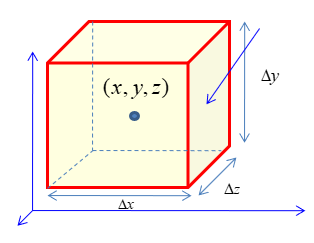
\includegraphics{微分推导守恒方程.jpg}
    \end{center}
    \caption{穿过单位面积面元的质量通量}
\end{figure}

给出的流体微团的体积可以表示为$\Delta  x\Delta y \Delta z$, 时间为$\Delta t$,流过的物理量通量可以表示为$F$,
从不同方向通过控制体的质量通量可以表示为$F_{\rho x}, F_{\rho y}, F_{\rho z}$,所以经过推导可以得到下面公式:
$$(\rho(t+\Delta t) - \rho(t))\Delta x \Delta y \Delta z + (\Delta F_{x\rho}\Delta y \Delta z+\Delta F_{y\rho}\Delta x \Delta z + \Delta F_{z\rho}\Delta x \Delta y)\Delta t = 0$$

从而可以得到质量的守恒方程,对于方程,我们左右同时除以$\Delta x \Delta y \Delta z \Delta t$, 同时将控制体的$\Delta x$等
趋于流体微团既可以得到$dx, dy, dz, dt$,从而得到如下公式:

$$\frac{\partial \rho}{\partial t} = -(\frac{\partial F_{x\rho}}{\partial x} + \frac{\partial F_{y\rho}}{\partial y}+\frac{\partial F_{z\rho}}{\partial z})$$

类似的,我们可以得到动量守恒方程和能量守恒方程:
$$\frac{\partial \bm{\theta}}{\partial t} = -(\frac{\partial F_{x\theta}}{\partial x} + \frac{\partial F_{y\theta}}{\partial y}+\frac{\partial F_{z\theta}}{\partial z})$$

$$\frac{\partial E}{\partial t} = -(\frac{\partial F_{xE}}{\partial x} + \frac{\partial F_{yE}}{\partial y}+\frac{\partial F_{zE}}{\partial z})$$

这里得到的一个结果是,通量的变化量,也就是散度是导致净通量变换的原因。
有一个非常中要的问题是要搞清楚这里的通量$F$在每个守恒公式中代表的意义。
顾名思义,这里的通量指的是单位时间通过单位面积面元的质量,动量,以及能量。
我们暂时只考虑$x$方向的面元,这里沿着$x$方向的速度为$u$,那么单位时间通过的质量
可以表示为
$$F_{\rho u} = \rho u \Delta t \Delta s$$
这里是单位面元,单位时间,所以可以得到沿着$x$方向的质量的通量为:$F_{\rho u} = \rho u$
同理,我们可以得到沿着其他两个方向的质量通量。

下面研究动量通量,首先给出关于动量与牛顿第二定律的若干定义:
\begin{equation*}
    \bm{p} = m \bm{v}
\end{equation*}
\begin{equation*}
    \bm{v} = \bm{v_0} +\bm{a}t
\end{equation*}

对动量得研究我们依旧沿着$x$轴方向,流场速度为$u$,所以可以得到如下公式:
\begin{equation*}
    \bm{F_{\theta x}} = \rho u \bm{V} + \bm{p}
\end{equation*}

其中第$\rho u \bm{V}$是流体质量自身携带得动量,但是同时质量得动量变化也与其受力有关,即
$m\Delta \bm{V} = \bm{F}\Delta t$,在单位时间内,动量得变化量就等于力本身。图1.3所示,为单位
面元受力情况,流体在这种情况下只受压力$\bm{p}$,所以得到上面得动量通量式子。

\begin{figure}[htbp]
    \begin{center}
        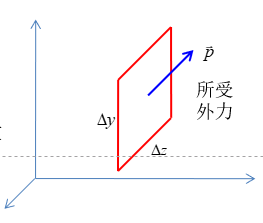
\includegraphics{通量.png}
    \end{center}
    \caption{动量通量受力图}
    
\end{figure}

需要弄明白其中$\bm{p}$得表示,即流动流体内部压强得分布,流动流体压强不同于静止流体,我们知道
静流体一点压强是水深得函数。但是流体流动,就会产生粘滞力,即流体得内摩擦力。从而在流体流动方向上压强
是不一样的。
\end{document}

